\section{Outils et technologie utilisées}


Lors de mon arrivé dans l'entreprise, j'ai du m'habitué à utiliser leurs outils de, gestion de projet, de communication, mais aussi de developement. Lors de nos projets d'études, là où on était une équipe de maximum 6 et on utilisait principalement des outils tels que Discord pour communiquer, VSCode pour developper, et GitHub Issue ou trello pour gérer le projet. Ici j'ai du m'habitué à utiliser des outils plus professionel et complet afin de pouvoir travailler sur des projets de plus grande taille. Voici la liste exhaustive de ces outils. 
\subsection{Outils}

\subsubsection{Monday}

Monday est un outil de gestion de projet simple qui permet de créer des tableaux et y ajouter des tâches.
Chaque tâche peut etre attribué à un quelqu'un, posséde un état (en cours, terminé, etc.) et une importance.
De plus chaque tâche posséde un espace "discussion" qui permet de faire état de l'avancement ou encore de noter certaines informations importantes. 

\begin{figure}[htbp]
    \center
    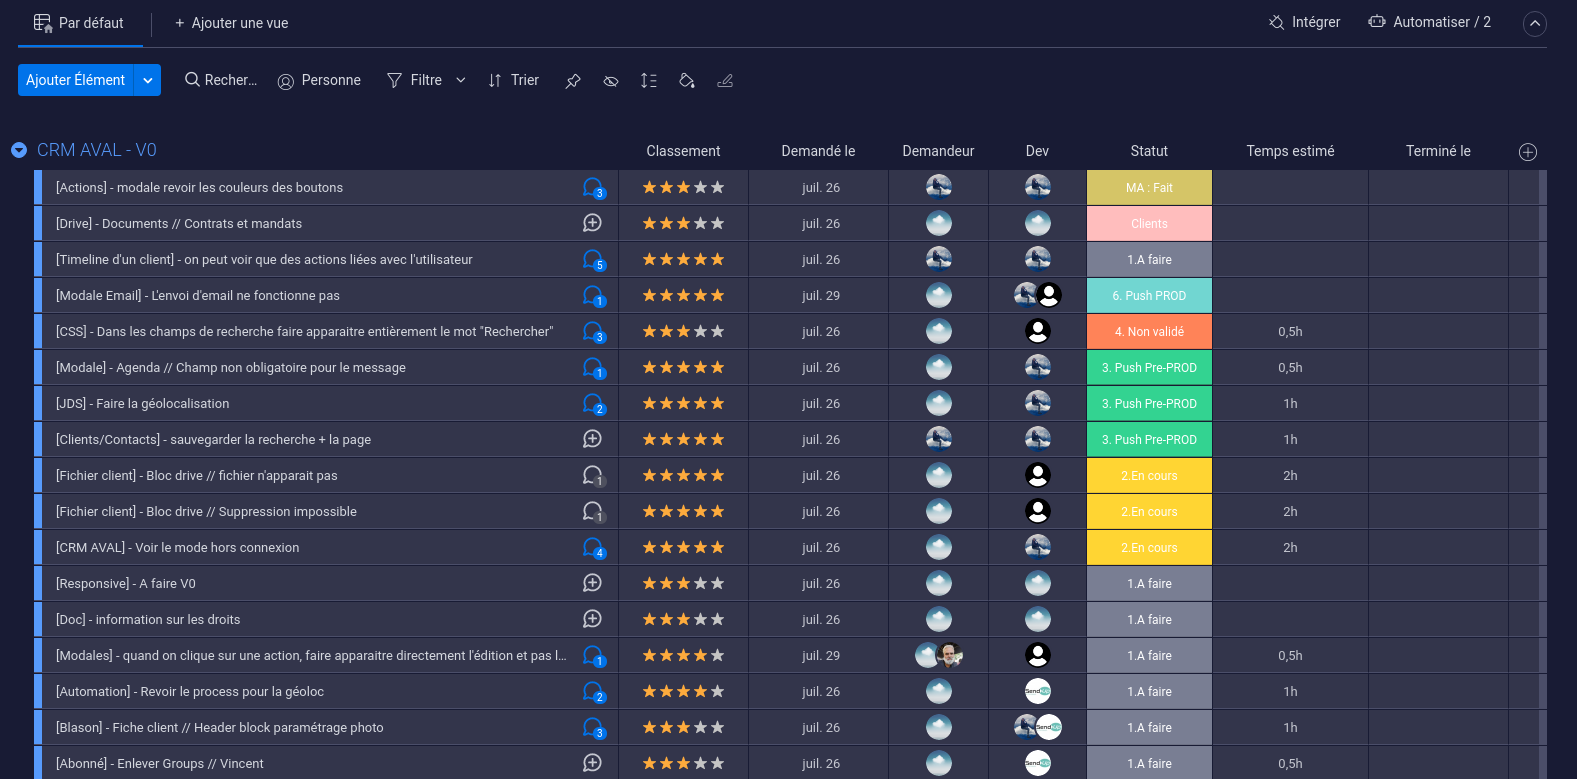
\includegraphics[width=\textwidth]{monday.png}
    \caption{Exemple de tableau Monday}
\end{figure}

\subsubsection{Google Workspace}
Afin de faciliter la communication au sein des équipes, l'entreprise utilise Google Workspace afin de produire de la documentation (Cahier des charges, etc...), GMail et Chat afin d'échanger rapidement et Agenda pour planifier les rendez-vous.
De plus, l'entreprise ayant des clients se trouvant dans toute la France, et tenant compte de la situation sanitaire actuelle  l'applications Google Meet est utilisée comme application de visio conférence, pour les diverses réunions et rendez-vous projets . 

\subsubsection{Git et GitKraken}
Git est un logiciel de gestion de version, il permet de créer des projets et de les versionner. Il permet également le partage du code ainsi que le développement sur plusieurs branches, afin de ne pas empiéter sur le travail des autres membres de l'équipe.

GitKraken lui est une interface graphique utilisant git. En effet git s'utilisant pricipalement par ligne de commande il est parfoit difficile de l'utiliser. GitKraken permet de faciliter l'utlisation de git et permet de tout faire en passant par l'interface (pull, merge, se déplacer entre les branche, etc..).

\begin{figure}[htbp]
    \center
    //TODO Screen GitKraken
\end{figure}

De plus il permet une totale intégration des git flow. C'est à dire créer facilement une branche par nouvelle feature, et simplement merge avec la branche de développement lorsque celle ci est terminée.
Les git flow permettent également une meilleure gestion des HotFix et des release mais je ne les ai pas utilisé lors de mon stage. 

\begin{figure}[htbp]
    \center
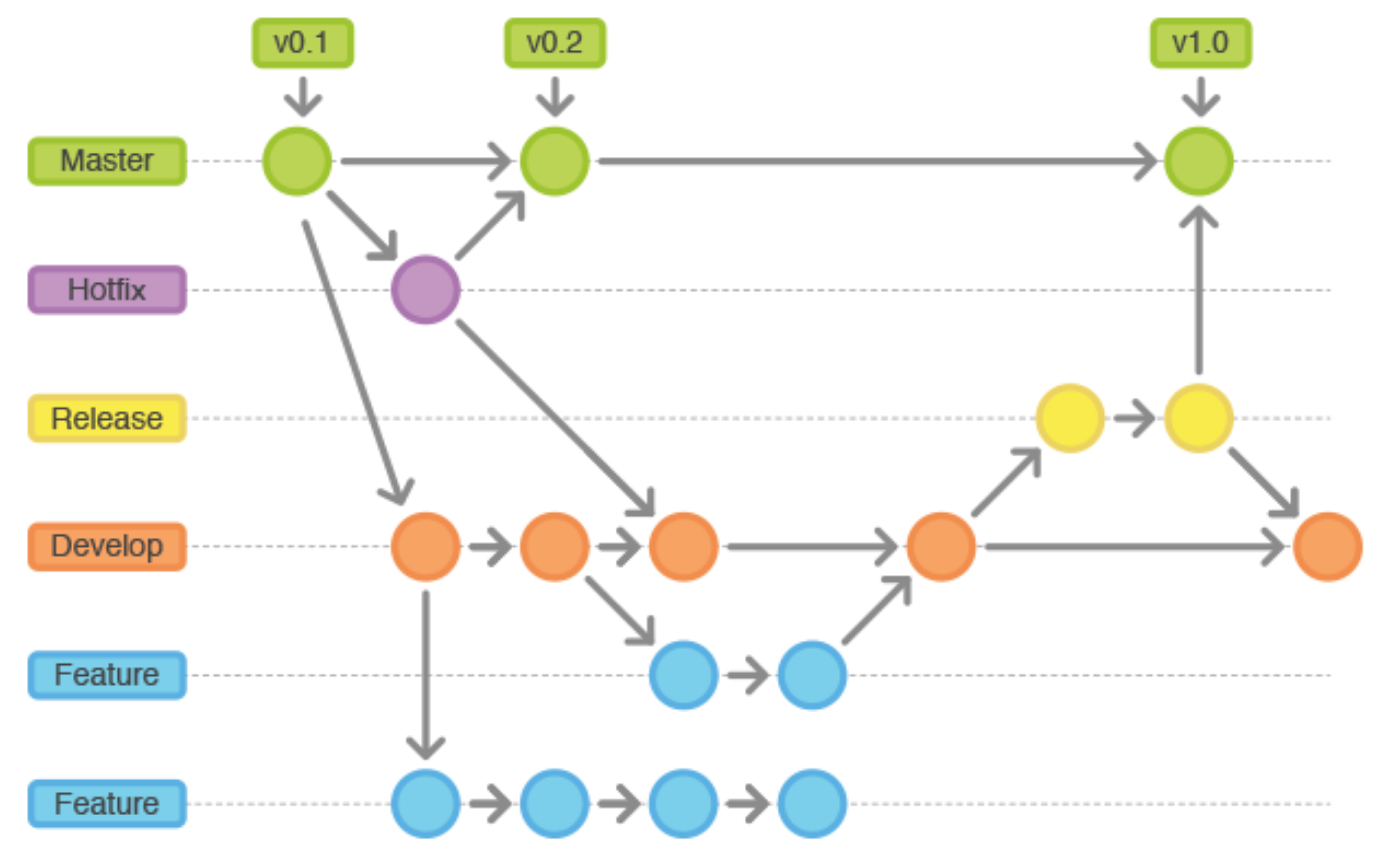
\includegraphics[width=0.5\textwidth]{gitflowimage.png}
\caption{Déroulement d'un git flow}
\end{figure}


\subsubsection{PHPStorm}

PHPStorm créé par JETBRAIN et l'un des IDE les plus complet pour développement web.
A l'aide de ses nombreux pluggins il permet une totale prise en charge des framework comme Symphony et VueJS. De plus il permet de facilement refactorer du code  ou encore de créer de nouveaux snippets afin de faciliter les phases de développement.
Malgré ses nombreux points positifs il est possible qu'il reste un peu dur à prendre en main au début mais par chance au cours de mes études supérieures j'ai été amené à utiliser InteliJ IDEA, ou encore Android studio qui sont deux IDE de JetBrain qui ont exactement la méme structure. 

\begin{figure}[htbp]
    \center 
    //TODO: Screen PHPStorm
\end{figure}


\subsubsection{Postman}

En ce moment l'entreprise ouvre son API de plus en plus à ces clients afin qu'il puissent eux même intégré les différents services de la platforme. Et c'est pour cette raison que l'API doit devenir de plus en plus robuste. Dans cette optique nous utilisons l'application Postman afin de facilement créer nos requêtes ainsi que des test associé. L'outils permet de faire hériter des tests à des sous collections ce qui nous permet de gagner du temps lorsque certains test sont génériques comme par exemple un temps de réponse inférieure à 200ms ou encore un statut de réponse différent de 500. 

\begin{figure}[htbp]
    \center
        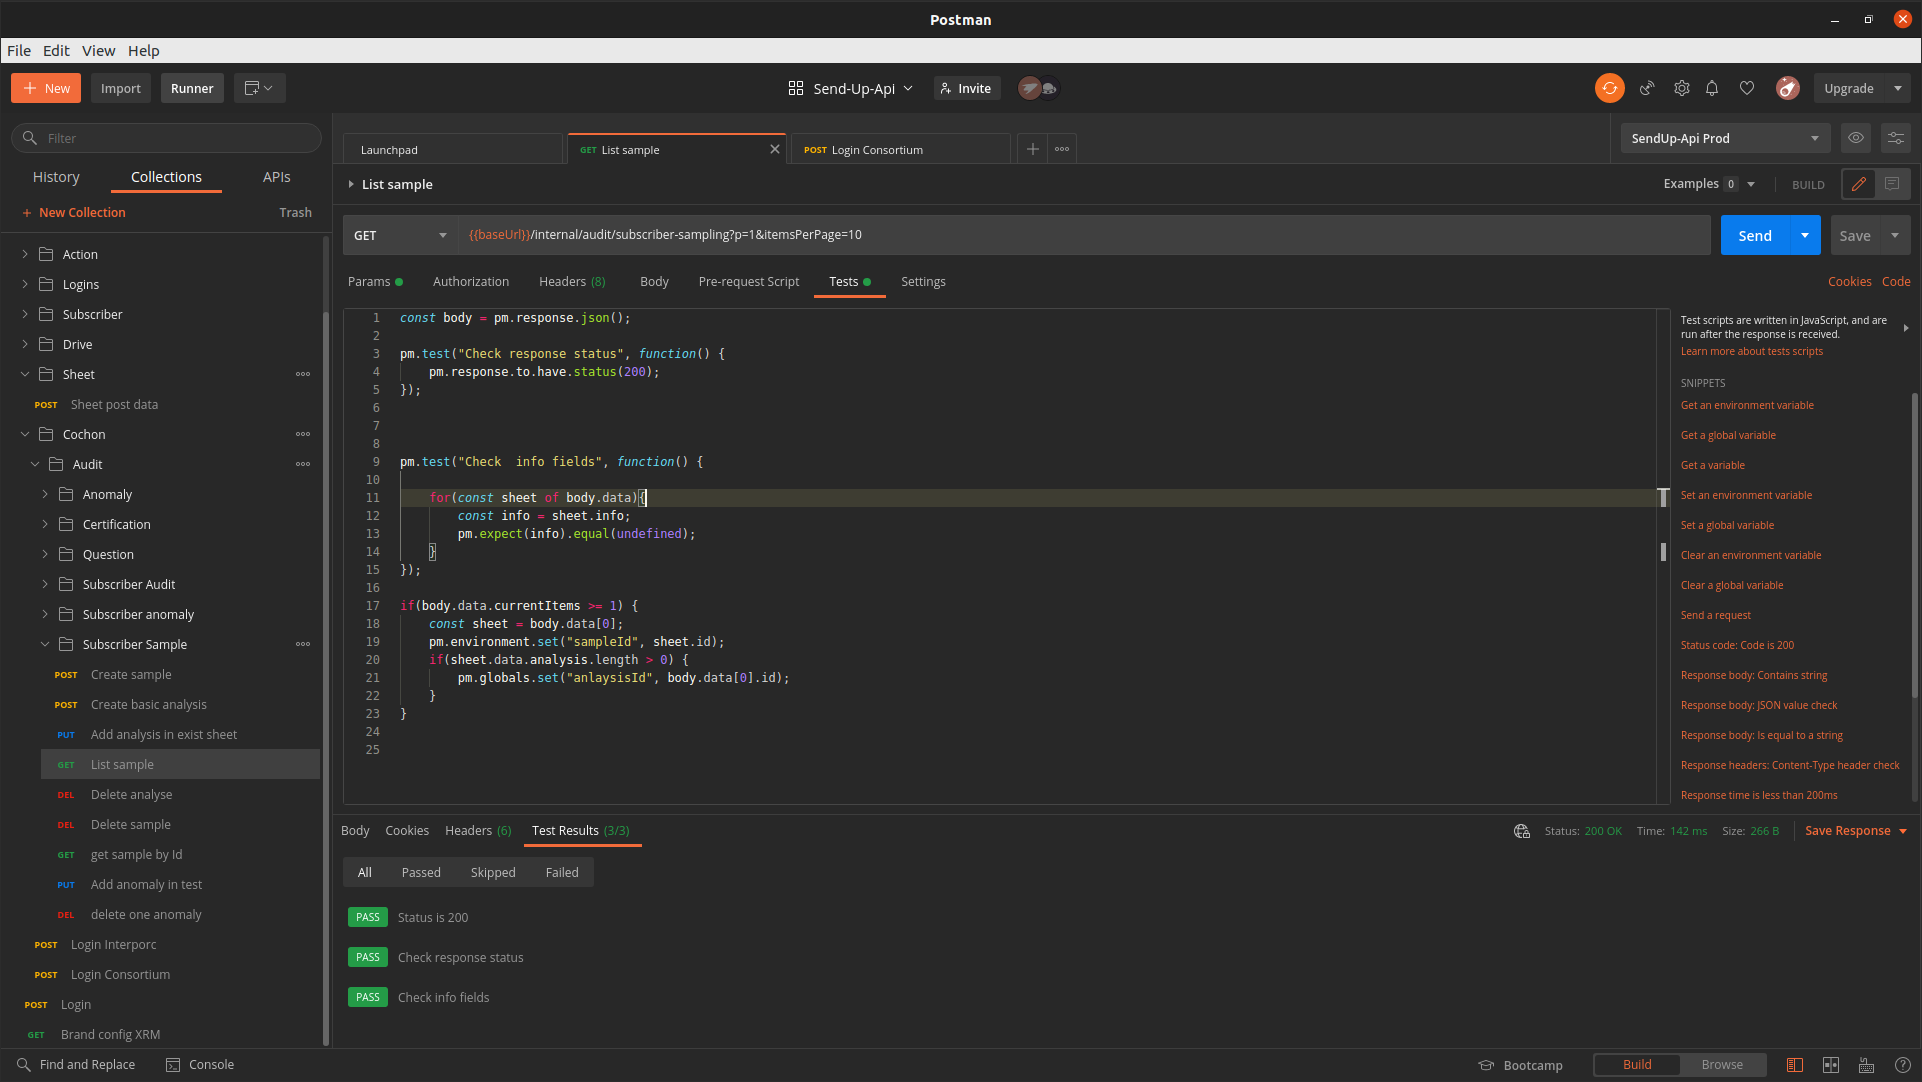
\includegraphics[width=\textwidth]{postman_test.png}
        \caption{Exemple de test Postman}
\end{figure}

De plus il intègre un \textit{collection runner} qui permet d'agencer l'ordre des requêtes, ainsi que de les lancer $x$ fois, à un intervalle de temps $y$. 

\begin{figure}[htbp]
    \center
    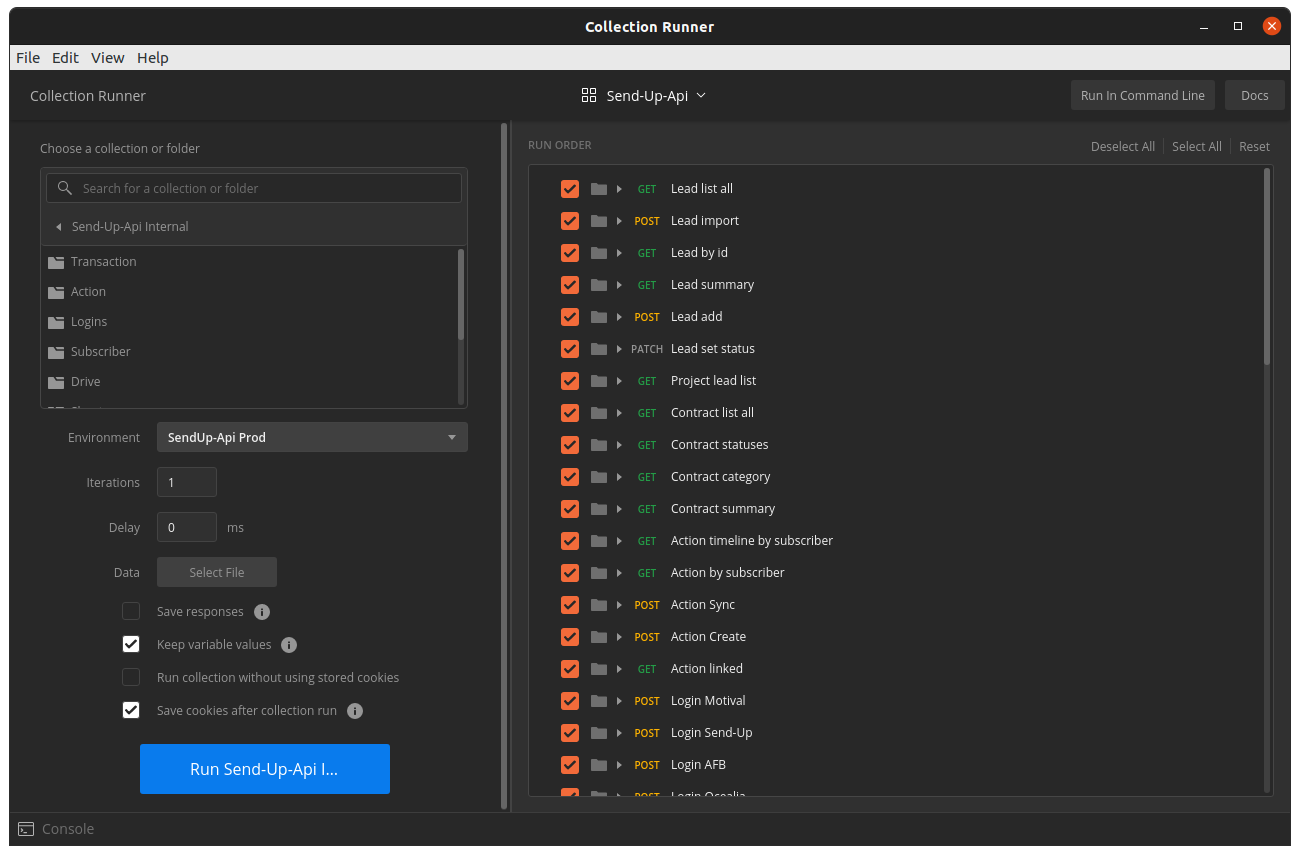
\includegraphics[width=\textwidth]{postman_collectionRunner.png}
    \caption{Exemple de collection runner Postman}
\end{figure}

\subsection{Technologies}

Historiquement la platforme Send-Up à était developé sur une stack Symphony 2.8/Jquery/Bootstrap. Aujourd'hui l'entreprise est en pleine transition technologique. Son objectif est de se passer de Jquery et Bootstrap au profit des nouvelles technologies du web et plus particulièrement du framework VueJS. Cette transition reste un défi pour l'entreprise car certains outils du site comme le \textit{studio digital} doivent garder ce relicat afin de garder une rétro-compatibilité mais aussi afin de facilité son usage auprés des clients. Voyons plus en détails les technologies choisies par l'entreprise à savoir Symfony et VueJS.

\subsubsection{Symfony}
Symfony est un framework PHP français développée en 2005 par Fabien Potencier. Basé sur le pattern Modèle-Vue-Controller, il est actuellement en version 5.x.x  Le gros avantage de Symfony sur les autres framework php du même type comme Laravel, ou CakePHP est sa documentation qui en plus d'être riches et également traduite en français. De plus, il possède une communauté trés importante et réactive. En effet a ce jour il existe plus de $X$ bundle sur la version 2.8. Et énormement de réponses sur les forums de developpeur.


\subsubsection{VueJS}
Pour remplacer la partie Jquery de Send-Up le framework VueJs a était choisi par l'équipe. Il s'agit d'un framework open-source développer à l'origine par Evan You en 2013. Ce framework facilite la création d'interface graphique et de Single Page Application (SPA). Pour présenter rapidement le framework voici un exemple de composant basique. 


Un fichier .vue est composé de 3 élements principaux.
\begin{itemize}
    \item \textbf{template} : contient le code HTML de l'interface graphique.
    \item \textbf{script} : contient la logique et le comportement du composant. 
    \item \textbf{styles} : contient les styles CSS du composant. Le style peux être utilisé avec une props \textit{scoped} afin de limiter les styles à l'intérieur du composant.
\end{itemize}

